\chapter{Diferensiasi Sel: Sel Otot Rangka}\label{ch:b2:cell-differentiation}

Sehelai \omterm{def:b2:cell-differentiation:myogenesis}{serabut otot} paha Anda adalah satu sel sepanjang tiga puluh
sentimeter, berinti ratusan, dan terjejali tongkat kontraktil dari ujung
ke ujung yang begitu teratur sehingga ia tampak bergaris di bawah
mikroskop. Ia bermula sebagai segerombol sel berpenampilan biasa yang
merangkak keluar dari sebuah somit, berlipat ganda, berhenti membelah,
berbaris, melebur, lalu menyalakan beberapa ratus gen yang belum pernah
dipakainya. Tiap sel tubuhnya memiliki genom yang sama; sebuah \omterm{def:b2:cell-differentiation:myogenesis}{serabut
otot} adalah apa yang dikerjakan genom itu ketika satu \omterm{prop:b2:cell-differentiation:transcriptional}{faktor
transkripsi} tertentu dinyalakan. Bab ini mengambil sel otot rangka
sebagai contoh kerja \emph{\omterm{def:b2:cell-differentiation:differentiation}{diferensiasi}} --- bagaimana sebuah sel
memperoleh dan mempertahankan sebuah jati diri yang terkhusus --- dan
sel otot adalah contoh yang baik karena sakelar induknya dikenal,
langkahnya dapat disaksikan di dalam cawan, dan sel jadinya adalah
sebuah mesin yang bagiannya terlihat.

\section{Apa itu diferensiasi}

\begin{definition}[Diferensiasi, determinasi, potensi]\label{def:b2:cell-differentiation:differentiation}
\index{diferensiasi}\index{determinasi}\index{sel punca}\index{potensi}
Sebuah sel disebut \emph{terdiferensiasi} ketika ia mengungkapkan pola
gen yang mantap --- dan dengan demikian protein, bentuk, serta
fungsi --- satu tipe sel. Ia \emph{terdeterminasi} (atau terpancang)
ketika nasibnya dipancangkan meskipun diferensiasinya belum mulai:
sebuah \omterm{def:b2:cell-differentiation:myogenesis}{mioblas} tampak seperti sebuah fibroblas tetapi hanya akan
membuat otot. \emph{Potensi} adalah rentang tipe yang masih dapat
diberikan sebuah sel: \emph{totipoten} (zigot dan blastomer
pertamanya, yang membuat segalanya termasuk \omterm{def:b2:mammal-reproduction:placenta}{plasentanya}),
\emph{pluripoten} (\omterm{def:b2:mammal-reproduction:implantation}{massa sel dalamnya}, yang membuat tiap jaringan
tubuhnya), \emph{multipoten} (sel punca darah atau otot, yang membuat
tipe satu jaringan), \emph{unipoten}. Sebuah \emph{sel punca} adalah
sel yang membelah untuk memberi satu anak seperti dirinya dan satu anak
yang lalu berdiferensiasi, dan itu mempertahankan persediaannya sembari
memasok jaringannya. Pada sebagian besar kasus, diferensiasi bukanlah
kehilangan gen melainkan sebuah pilihan di antaranya: genom sebuah inti
otot tetap lengkap.
\end{definition}
\begin{proof}[Bukti eksperimental]
Gurdon (1962) memindahkan nukleus sebuah sel usus berudu yang
terdiferensiasi ke dalam sebutir telur katak yang nukleusnya sendiri
telah dimusnahkan; sebagian telurnya berkembang menjadi katak yang
normal dan subur. Nukleus yang terdiferensiasi itu tidak kehilangan
satu pun gen yang dibutuhkan untuk membuat seekor hewan utuh;
sitoplasma telurnya telah menyetelnya ulang. Operasi yang sama dengan
nukleus sebuah sel kelenjar susu di dalam sebutir telur domba
menghasilkan Dolly (1996), dan pemrograman ulang sebuah fibroblas kulit
menjadi \omterm{def:b2:cell-differentiation:differentiation}{sel punca} pluripoten oleh empat \omterm{prop:b2:cell-differentiation:transcriptional}{faktor transkripsi} (Yamanaka,
2006) menunjukkan bahwa penyetelan ulangnya dapat dikerjakan dengan
segelintir protein.
\end{proof}

\begin{proposition}[Diferensiasi bersifat transkripsi]\label{prop:b2:cell-differentiation:transcriptional}
\index{faktor transkripsi}\index{pengatur induk}
Perbedaan antara dua tipe sel terletak pada gen mana yang
ditranskripsi. Beberapa \emph{\omterm{prop:b2:cell-differentiation:transcriptional}{faktor transkripsi}}, yang diungkapkan
sebagai tanggapan terhadap isyarat pengimbas
\cref{ch:b2:vertebrate-development}, mengikat daerah pengatur ratusan
gen sasarannya lalu menyalakannya, sementara gen nasib lainnya
dimatikan; dan karena faktor semacam itu lazimnya mengaktifkan gennya
sendiri, keadaannya, begitu dimasuki, mempertahankan dirinya sendiri.
Bagi sebagian jaringan, satu faktor tunggal menjadi sebuah
\emph{\omterm{prop:b2:cell-differentiation:transcriptional}{pengatur induk}} yang mencukupi untuk memaksakan nasibnya pada
sel bertipe lain: \omterm{def:b2:cell-differentiation:myogenesis}{MyoD} bagi otot rangka, Pax6 bagi mata, Sox9 bagi
rawan. Keadaannya dimantapkan lebih jauh oleh perubahan pada
kromatinnya --- metilasi DNA, pengubahan histon --- yang menjaga gen
yang dibungkam tetap bisu sepanjang pembelahannya (yaitu
\emph{epigenetika} jilid Tahun ke-3). Maka sebuah sel yang
terdiferensiasi mengingat dirinya siapa tanpa perubahan apa pun pada
urutan DNA-nya, dan ingatannya ditulis dalam pola faktor dan
kromatinnya, bukan di dalam gennya.
\end{proposition}

\section{Pembuatan sehelai serabut otot}

\begin{definition}[Miogenesis]\label{def:b2:cell-differentiation:myogenesis}
\index{mioblas}\index{miotuba}\index{serabut otot}\index{MyoD}
Di dalam lembaganya, sel dermomiotom somitnya diimbas isyarat dari
\omterm{prop:b2:vertebrate-development:neurulation}{tabung saraf}, notokord, dan ektoderm permukaannya untuk mengungkapkan
faktor miogeniknya \emph{MyoD} dan \emph{Myf5}: mereka kini menjadi
\emph{mioblas}, yang terdeterminasi tetapi masih membelah dan tidak
istimewa penampilannya. Mioblasnya bermigrasi --- ke dalam \omterm{def:b2:limb-organogenesis:bud}{tunas
tungkainya}, misalnya --- lalu berlipat ganda selama faktor pertumbuhan
(FGF) hadir. Ketika faktornya habis, mereka menarik diri dari daur
selnya, mengungkapkan faktor kedua, yaitu \emph{miogenin}, berbaris
ujung ke ujung, lalu \emph{melebur}: membrannya menyatu menjadi satu
\emph{miotuba} panjang dengan banyak inti berderet. Miotubanya
menyalakan gen ototnya --- aktin, miosin, troponin, tropomiosin,
kreatin kinase, reseptor asetilkolin --- merakit perangkat
kontraktilnya, lalu matang menjadi sehelai \emph{serabut otot} yang
intinya terletak di tepinya. Sehelai serabut tidak pernah membelah
lagi; beberapa mioblas tetap tinggal di sebelahnya, diam, sebagai
\emph{sel satelit}, yaitu \omterm{def:b2:cell-differentiation:differentiation}{sel punca} yang memperbaiki serta
menumbuhkan ototnya seumur hidup.
\end{definition}

\begin{omfigure}
\begin{tikzpicture}[every node/.style={font=\scriptsize}, >=stealth]
  % somite
  \draw[thick, fill=omProp!25] (0,0) ellipse (0.6 and 0.5); \node[below, align=center] at (0,-0.6) {somit\\(dermomiotom)};
  \draw[->, thick] (0.7,0) -- (1.6,0) node[midway, above=0.35cm, align=center] {pengimbasan\\Wnt, Shh};
  % myoblasts dividing
  \foreach \p in {(2.2,0.3),(2.7,-0.3),(3.2,0.3),(3.7,-0.3)} \draw[thick, fill=omDef!25] \p ellipse (0.28 and 0.18);
  \node[below, align=center] at (3.0,-0.6) {mioblas: MyoD, Myf5\\membelah selagi FGF hadir};
  \draw[->, thick] (4.1,0) -- (5.0,0) node[midway, above=0.45cm, align=center] {FGF ditarik:\\miogenin,\\keluar dari daurnya};
  % aligned, fusing
  \foreach \x in {5.35,5.95,6.55,7.15} \draw[thick, fill=omDef!25] (\x,0) ellipse (0.3 and 0.16);
  \node[below, align=center] at (6.25,-0.6) {berbaris lalu melebur};
  \draw[->, thick] (7.6,0) -- (8.5,0);
  % myotube
  \draw[thick, fill=omDef!15, rounded corners=6pt] (8.7,-0.3) rectangle (12.6,0.3);
  \foreach \x in {9.2,10.0,10.8,11.6,12.3} \fill[omDef!80!black] (\x,0) ellipse (0.13 and 0.08);
  \node[below, align=center] at (10.65,-0.6) {miotuba: banyak inti,\\gen otot menyala, miofibril dirakit};
\end{tikzpicture}

{\small Miogenesis: sel somit yang terimbas menjadi \omterm{def:b2:cell-differentiation:myogenesis}{mioblas} yang
membelah; ketika faktor pertumbuhannya ditarik mereka berhenti
membelah, berbaris, lalu melebur menjadi sebuah \omterm{def:b2:cell-differentiation:myogenesis}{miotuba} berinti banyak
yang menyalakan gen ototnya.}
\end{omfigure}

\begin{omfigure}
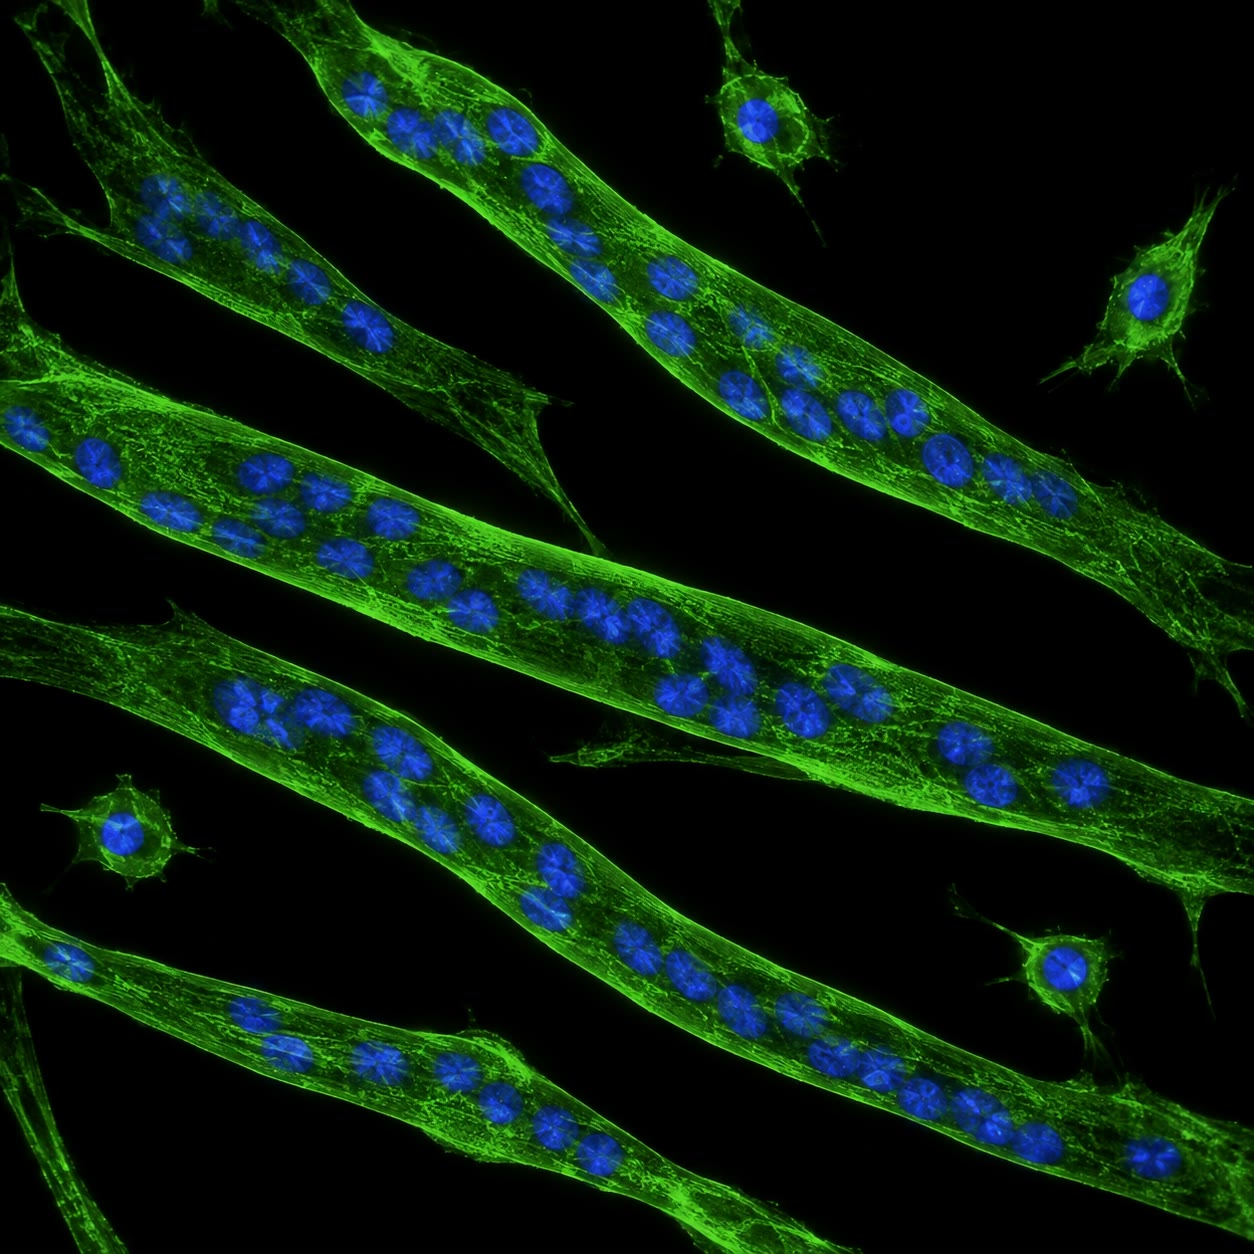
\includegraphics[width=0.44\linewidth]{images/book4/ai/b4-12-myotubes.jpg}\hspace{0.04\linewidth}
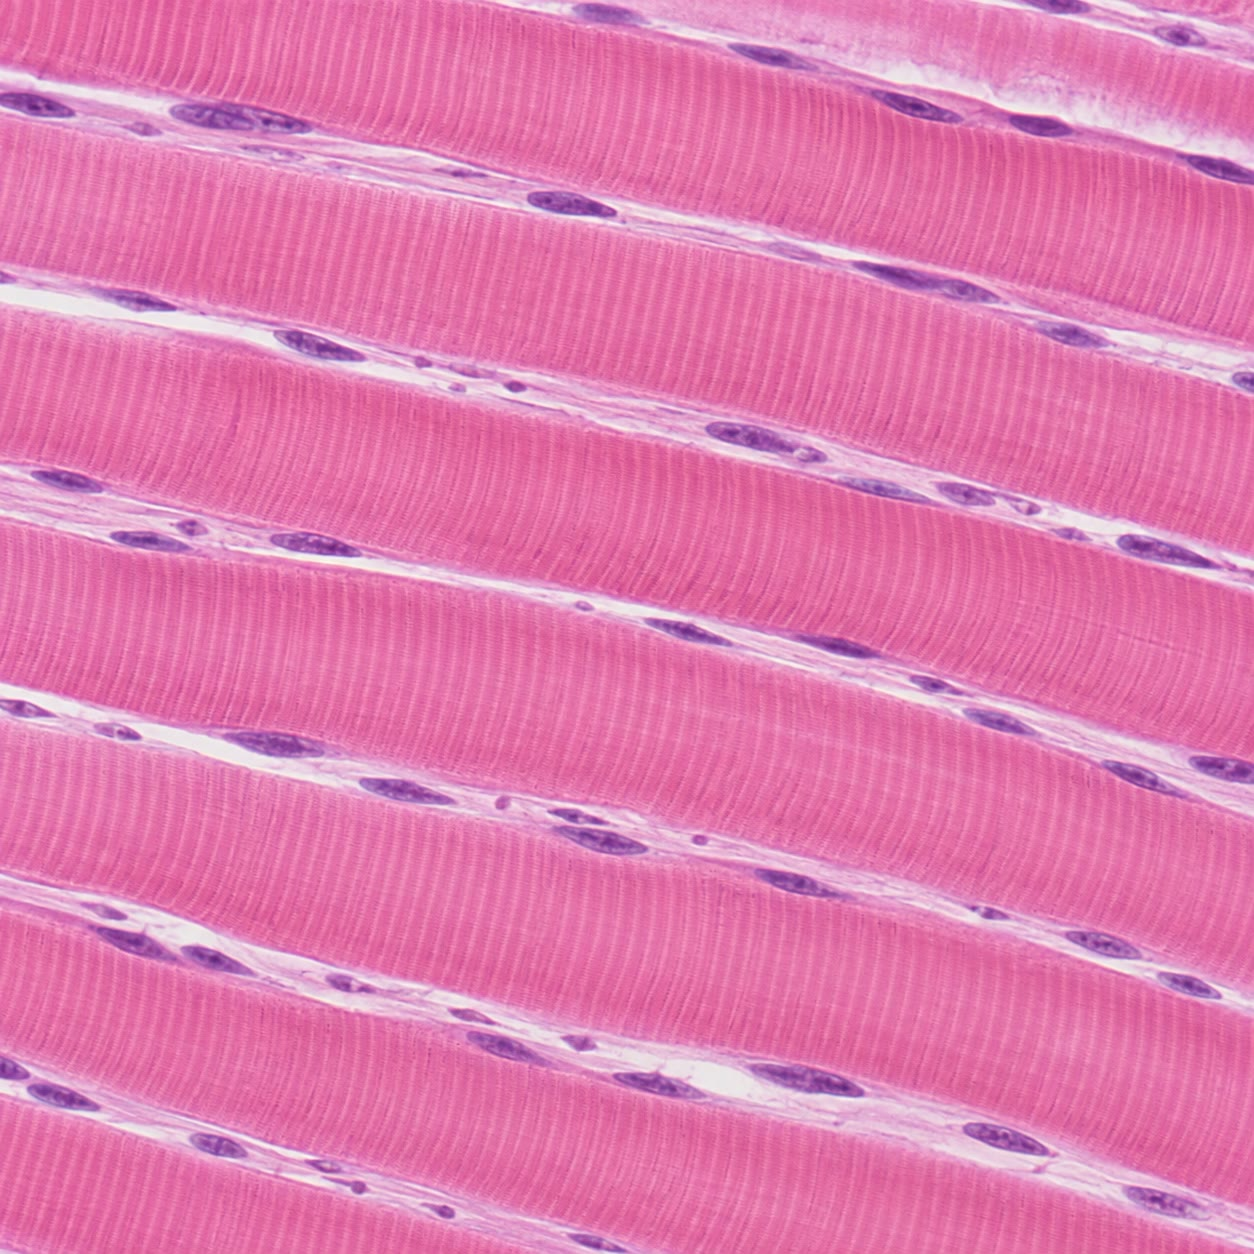
\includegraphics[width=0.44\linewidth]{images/book4/ai/b4-12-muscle-fibres.jpg}

{\small Kiri: \omterm{def:b2:cell-differentiation:myogenesis}{miotuba} di dalam biakan, masing-masing sebuah sel hasil
peleburan dengan deretan inti, di samping \omterm{def:b2:cell-differentiation:myogenesis}{mioblas} tunggal yang belum
melebur. Kanan: serabut matang dilihat membujur, garis lintangnya
adalah \omterm{def:b2:cell-differentiation:fibre}{sarkomer} yang berulang dan intinya terdorong ke tepinya.}
\end{omfigure}

\begin{proposition}[MyoD: sebuah sakelar induk]\label{prop:b2:cell-differentiation:myod}
\index{pengatur induk!MyoD}
\omterm{def:b2:cell-differentiation:myogenesis}{MyoD} adalah sebuah \omterm{prop:b2:cell-differentiation:transcriptional}{faktor transkripsi} keluarga heliks-gelung-heliks. Ia
mengikat, sebagai sebuah dimer bersama sebuah protein pasangan yang
ada di mana-mana, sebuah urutan enam basa (kotak E, CANNTG) di dalam
daerah pengatur gen ototnya, merekrut enzim pembuka kromatin, lalu
menyalakan gennya --- termasuk gen bagi miogenin dan bagi \omterm{def:b2:cell-differentiation:myogenesis}{MyoD} sendiri,
dan begitulah keadaannya bertahan. Kegiatannya digerbangi: di dalam
\omterm{def:b2:cell-differentiation:myogenesis}{mioblas} yang membelah, sebuah protein penghambat (Id), yang diimbas
faktor pertumbuhannya, menyita pasangannya lalu menjaga \omterm{def:b2:cell-differentiation:myogenesis}{MyoD} tetap
menganggur; ketika faktor pertumbuhannya ditarik, Id-nya lenyap dan
\omterm{def:b2:cell-differentiation:myogenesis}{MyoD} bekerja. Karena \omterm{def:b2:cell-differentiation:myogenesis}{MyoD} mencukupi untuk memaksakan program ototnya
pada sebuah fibroblas, sebuah sel lemak, atau sebuah sel saraf, nasib
ototnya, dalam arti tertentu, hanya sedalam satu gen: kesukaran menjadi
sebuah otot bukanlah dalam mengetahui caranya, melainkan dalam
diperintah untuk itu.
\end{proposition}
\begin{proof}[Bukti eksperimental]
Davis, Weintraub, dan Lassar (1987) memindahkan satu cDNA tunggal, yang
diisolasi dari \omterm{def:b2:cell-differentiation:myogenesis}{mioblas}, ke dalam fibroblas biakan: fibroblasnya
berhenti membelah, melebur menjadi \omterm{def:b2:cell-differentiation:myogenesis}{miotuba}, lalu membuat protein otot.
Gennya diberi nama \omterm{def:b2:cell-differentiation:myogenesis}{MyoD}. Kerabatnya Myf5, miogenin, dan MRF4 ditemukan
lewat kehomologan; seekor mencit yang tidak memiliki \omterm{def:b2:cell-differentiation:myogenesis}{MyoD} maupun Myf5
tidak bermioblas dan sama sekali tidak berotot rangka, sedangkan mencit
yang tidak memiliki miogenin memiliki \omterm{def:b2:cell-differentiation:myogenesis}{mioblas} yang tidak pernah melebur.
\end{proof}

\begin{theorem}[Sebuah sakelar yang menopang dirinya]\label{thm:b2:cell-differentiation:switch}
\index{kedwimantapan}\index{umpan balik positif!gen}
Misalkan $m$ adalah jumlah sebuah faktor yang mengaktifkan gennya
sendiri dengan tanggapan yang bekerja sama (sigmoid) dan terurai pada
laju $k$:
\[
\frac{\mathrm{d}m}{\mathrm{d}t} = \frac{a\,m^{2}}{K^{2} + m^{2}} + b - k\,m,
\]
dengan $b$ sebagai sintesis basal yang kecil. Bagi $a$, $b$, $K$, dan
$k$ yang sesuai, persamaan ini memiliki \emph{dua} keadaan tunak yang
mantap, satu yang rendah mendekati $b/k$ dan satu yang tinggi mendekati
$a/k$, yang dipisahkan sebuah ambang yang tak mantap: selnya bersifat
\emph{dwimantap}. Sebuah isyarat pengimbas yang sementara, yang
mendorong $m$ di atas ambangnya, mengirim selnya ke keadaan tingginya,
dan ia tinggal di situ sesudah isyaratnya pergi; di bawah ambangnya ia
kembali ke keadaan rendahnya. Inilah sebuah ingatan yang dibangun dari
sebuah gelung umpan balik, dan itulah sebabnya sebuah sel, begitu
terpancang, tetap terpancang sepanjang pembelahannya dan tanpa
kehadiran pengimbasnya.
\end{theorem}
\begin{proof}
Keadaan tunaknya memenuhi $k m = a m^{2}/(K^{2} + m^{2}) + b$. Ruas
kanannya adalah sebuah sigmoid yang naik dari $b$ sampai $a + b$; ruas
kirinya adalah sebuah garis lewat titik asal dengan kemiringan $k$.
Bagi $b/k < K$ dan $k$ yang cukup kecil sehingga garisnya memotong
bagian curam sigmoidnya, kedua kurvanya berpotongan tiga kali: pada
$m_{\text{rendah}} \approx b/k$, pada $m_{\text{u}}$ yang di tengah,
dan pada $m_{\text{tinggi}} \approx (a +
b)/k$. Kemantapannya: di bawah
$m_{\text{rendah}}$ sintesisnya melampaui peluruhannya dan $m$ naik;
antara $m_{\text{rendah}}$ dan $m_{\text{u}}$ peluruhannya melampaui
sintesisnya dan $m$ turun kembali; antara $m_{\text{u}}$ dan
$m_{\text{tinggi}}$ sintesisnya melampaui peluruhannya dan $m$ memanjat
ke $m_{\text{tinggi}}$; di atasnya, $m$ turun kembali ke
$m_{\text{tinggi}}$. Maka kedua yang terluar mantap, yang di tengah tak
mantap dan menjadi ambangnya.
\end{proof}

\begin{omfigure}
\begin{tikzpicture}
\begin{axis}[
  width=0.74\linewidth, height=5.8cm,
  axis x line=bottom, axis y line=left,
  xmin=0, xmax=4, ymin=0, ymax=1.3,
  xlabel={kadar faktornya $m$ (relatif)}, ylabel={laju},
  xlabel style={font=\small, at={(axis description cs:0.5,-0.12)}, anchor=north},
  ylabel style={font=\small},
  tick label style={font=\small}, xtick={0,1,2,3,4}, ytick={0,0.5,1},
  legend style={font=\scriptsize, at={(0.03,0.97)}, anchor=north west, draw=none},
  clip=false,
]
\addplot[very thick, omDef, domain=0:4, samples=100] {x^2/(1+x^2) + 0.02};
\addlegendentry{sintesis: $a m^2/(K^2 + m^2) + b$}
\addplot[very thick, omThm, domain=0:3.2, samples=2] {0.4*x};
\addlegendentry{penguraian: $k m$}
\fill[omDef] (axis cs:0.055,0.022) circle (2pt); \draw[gray] (axis cs:0.08,0.04) -- (axis cs:0.33,0.42); \node[font=\scriptsize, anchor=west] at (axis cs:0.35,0.45) {padam};
\draw[gray, thick] (axis cs:0.41,0.164) circle (2pt); \node[font=\scriptsize, anchor=west] at (axis cs:0.55,0.10) {ambang};
\fill[omDef] (axis cs:2.1,0.84) circle (2pt); \node[font=\scriptsize, anchor=north] at (axis cs:2.1,0.78) {nyala};
\end{axis}
\end{tikzpicture}

{\small Sebuah sakelar dwimantap ($a = 1$, $K = 1$, $b = 0.02$, $k = 0.4$).
Sintesisnya (sigmoid) dan penguraiannya (garis) berpotongan tiga kali:
dua keadaan yang mantap, padam dan nyala, serta sebuah ambang tak
mantap di antaranya. Sebuah isyarat yang mengangkat $m$ melewati
ambangnya memancangkan selnya pada keadaan nyala secara tetap.}
\end{omfigure}

\section{Sel jadinya}

\begin{definition}[Serabut otot]\label{def:b2:cell-differentiation:fibre}
\index{sarkomer}\index{miofibril}\index{retikulum sarkoplasma}\index{tubulus T}
Sehelai \omterm{def:b2:cell-differentiation:myogenesis}{serabut otot} rangka adalah sebuah silinder bergaris tengah
\qtyrange{10}{100}{\micro m} dan sepanjang sampai puluhan sentimeter,
yang dibatasi \emph{sarkolema}, dengan ratusan inti tepat di bawahnya.
Bagian dalamnya terisi \emph{miofibril} yang sejajar, dan masing-masing
adalah sebuah rantai \emph{sarkomer} sepanjang \qty{2.5}{\micro m}: di
antara dua cakram Z, filamen tipis aktin (beserta tropomiosin dan
troponin) yang tertambat pada cakram Z-nya berselang-seling dengan
filamen tebal miosin yang ditahan di pusatnya, dan pola tindihannya
memberi garis lintangnya. Di sekeliling tiap miofibrilnya, sebuah
renda \emph{retikulum sarkoplasma} menyimpan kalsium; \emph{tubulus
lintang}, yaitu lekukan sarkolemanya, berjalan di antara miofibrilnya
lalu mengusung isyarat listriknya dari permukaannya ke bagian dalamnya.
Mitokondria menjejali ruangnya, dan sitoplasmanya memuat glikogen,
kreatin fosfat, dan, pada serabut merahnya, mioglobin. Selnya dibangun
bagi satu hal --- memendek atas perintah --- dan permesinan perintah
itu adalah \cref{ch:b2:muscle-movement}.
\end{definition}

\begin{omfigure}
\begin{tikzpicture}[every node/.style={font=\scriptsize}]
  % a stretch of myofibril with two sarcomeres
  \foreach \s in {0,4.4} {
    \begin{scope}[xshift=\s cm]
      \draw[very thick, omThm] (0,-1.1) -- (0,1.1);
      \foreach \y in {-0.9,-0.5,-0.1,0.3,0.7} { \draw[thick, omDef] (0,\y) -- (1.6,\y); \draw[thick, omDef] (4.4,\y) -- (2.8,\y); }
      \foreach \y in {-0.7,-0.3,0.1,0.5,0.9} { \draw[line width=3pt, omExo!80!black] (1.0,\y) -- (3.4,\y); }
      \draw[gray] (2.2,-1.1) -- (2.2,1.1);
    \end{scope}
  }
  \draw[very thick, omThm] (8.8,-1.1) -- (8.8,1.1);
  \node[omThm, below] at (0,-1.15) {cakram Z};
  \node[omThm, below] at (4.4,-1.15) {cakram Z};
  \node[omThm, below] at (8.8,-1.15) {cakram Z};
  \node[omDef, above] at (0.8,1.15) {filamen tipis (aktin)};
  \node[omExo!80!black, above] at (6.6,1.15) {filamen tebal (miosin)};
  \node[gray, below] at (2.2,-1.15) {garis M};
  \draw[<->] (0,1.9) -- (4.4,1.9); \node[above] at (2.2,1.9) {satu sarkomer, \qty{2.5}{\micro m}};
  \draw[<->] (5.4,-1.6) -- (7.8,-1.6); \node[below] at (6.6,-1.6) {pita A (gelap)};
  \draw[<->] (7.8,-1.6) -- (9.8,-1.6); \node[below] at (8.8,-1.6) {pita I (terang)};
\end{tikzpicture}

{\small Dua \omterm{def:b2:cell-differentiation:fibre}{sarkomer} sebuah \omterm{def:b2:cell-differentiation:fibre}{miofibril}: filamen tipis aktin yang
tertambat pada cakram Z-nya berselang-seling dengan filamen tebal
miosin yang berpusat pada garis M-nya. Tindihannya memberi pita A yang
gelap dan pita I yang terang pada garis lintangnya.}
\end{omfigure}

\begin{proposition}[Tipe serabut]\label{prop:b2:cell-differentiation:types}
\index{tipe serabut otot}
Sebuah otot adalah campuran tipe serabut, yang sebagian ditetapkan
garis keturunan \omterm{def:b2:cell-differentiation:myogenesis}{mioblasnya} dan sebagian lagi oleh saraf yang
mempersarafi serabutnya. Serabut \emph{oksidatif lambat} (tipe I)
memiliki miosin yang lambat, banyak mitokondria dan kapiler, serta
mioglobin --- merah, tak kenal lelah, dibangun bagi sikap tubuh dan
ketahanan. Serabut \emph{glikolitik cepat} (tipe IIx) memiliki miosin
yang cepat, sedikit mitokondria, dan banyak glikogen --- putih,
bertenaga, dan habis dalam semenit. Serabut \emph{oksidatif cepat}
(tipe IIa) terletak di antaranya. Betis seorang pelari cepat sebagian
besar serabut cepat, betis seorang pelari maraton sebagian besar
serabut lambat, dan perbandingannya terwariskan; tetapi tipenya tidak
tetap: mempersarafi silang sebuah otot cepat dengan sebuah saraf
lambat, atau berbulan-bulan latihan ketahanan, mengubah serabutnya ke
arah tipe lambat, karena pola impuls sarafnya menyalakan gen isoform
miosinnya dan gen biogenesis mitokondrianya. Sebuah sel yang
terdiferensiasi mempertahankan jati dirinya sebagai \omterm{def:b2:cell-differentiation:myogenesis}{serabut otot} dan
tetap saja merevisi programnya sebagai tanggapan terhadap pemakaiannya.
\end{proposition}

\begin{example}[Pertumbuhan dan perbaikan]\label{ex:b2:cell-differentiation:satellite}
Sebuah otot tumbuh pada orang dewasa bukan dengan menambahkan serabut
melainkan dengan membesarkannya: latihan menambahkan \omterm{def:b2:cell-differentiation:fibre}{miofibril} pada
tiap serabutnya, dan \emph{sel satelit} melebur ke dalamnya untuk
memasok inti tambahan yang dibutuhkan sitoplasma yang lebih besar.
Sesudah cedera, sel yang sama membelah, mengungkapkan kembali \omterm{def:b2:cell-differentiation:myogenesis}{MyoD},
melebur, lalu membangun kembali ruas yang rusak dalam beberapa pekan
--- program lembaganya dijalankan lagi pada orang dewasa. Pada distrofi
otot, serabutnya tidak memiliki distrofin, yaitu sebuah protein yang
mengikatkan \omterm{def:b2:cell-differentiation:fibre}{miofibrilnya} pada membrannya, lalu robek selama
pengerutannya; sel satelitnya memperbaikinya berulang-ulang sampai,
sesudah bertahun-tahun, persediaannya habis dan jaringan berserat
mengambil tempat ototnya.
\end{example}

\begin{omfigure}
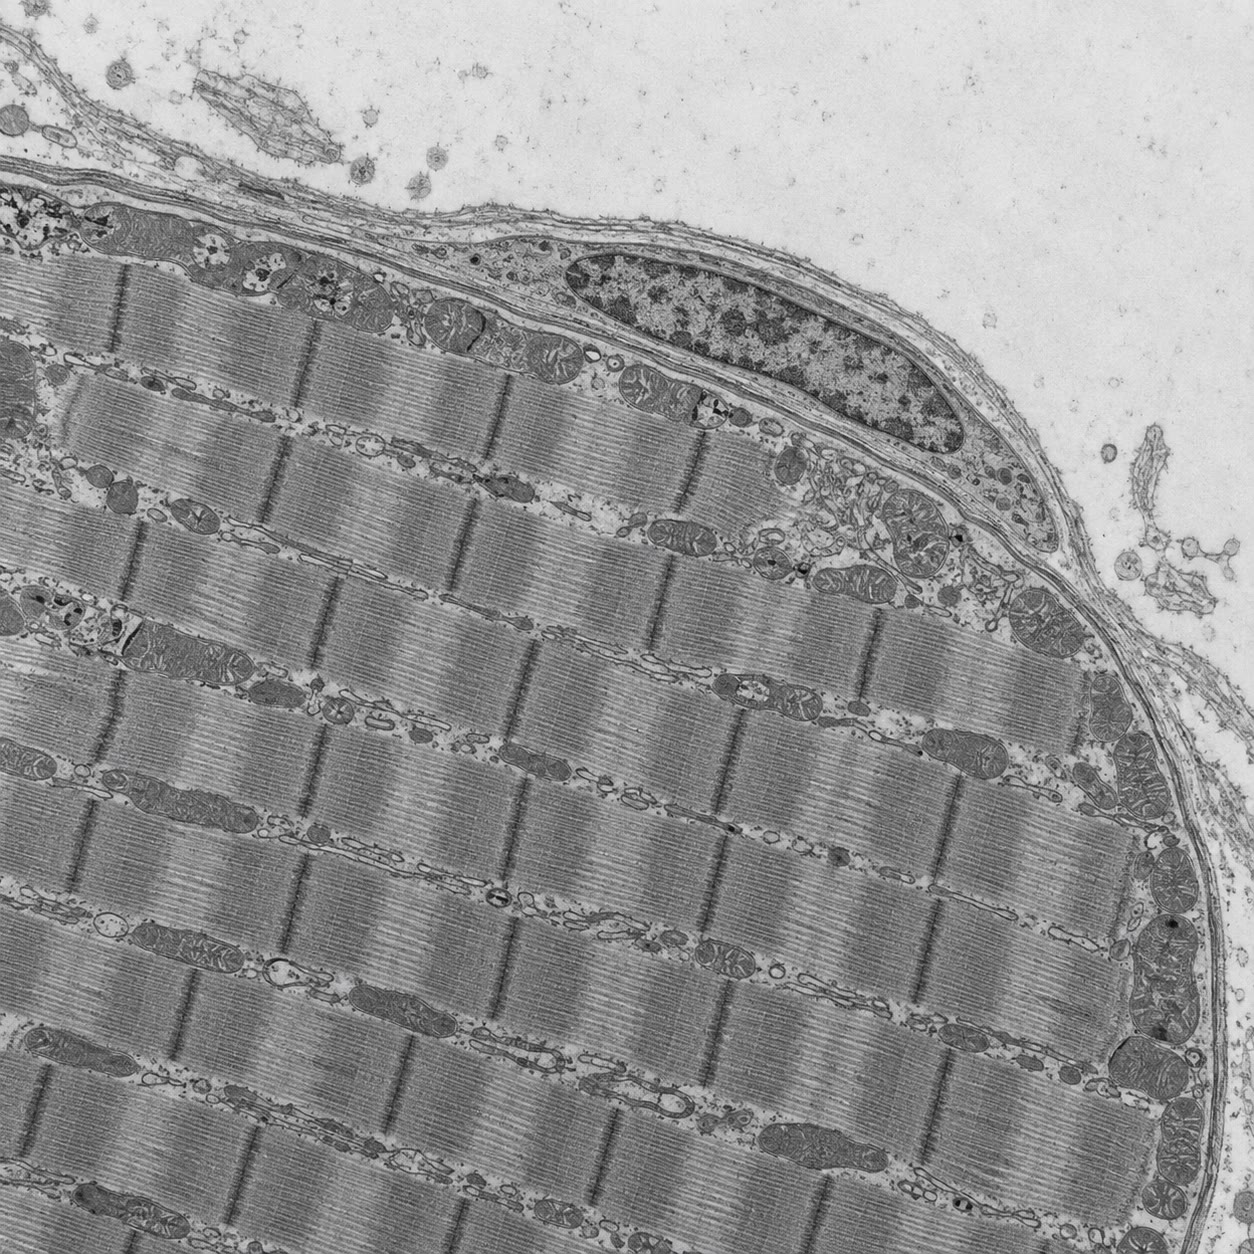
\includegraphics[width=0.42\linewidth]{images/book4/ai/b4-12-satellite-cell-tem.jpg}

{\small Sebuah sel satelit di bawah mikroskop elektron: sebuah sel
kecil berinti tunggal yang terselip di antara membran sehelai \omterm{def:b2:cell-differentiation:myogenesis}{serabut
otot} dan lamina basalnya --- yaitu cadangan \omterm{def:b2:cell-differentiation:myogenesis}{mioblas} serabutnya.}
\end{omfigure}

\section{Latihan}

\begin{exercise}[$\star$]\label{exo:b2:cell-differentiation:1}
Definisikan \omterm{def:b2:cell-differentiation:differentiation}{diferensiasi}, \omterm{def:b2:cell-differentiation:differentiation}{determinasi}, dan \omterm{def:b2:cell-differentiation:differentiation}{potensi}, lalu tempatkan
zigotnya, sebuah sel \omterm{def:b2:mammal-reproduction:implantation}{massa sel dalam}, sebuah sel satelit, dan sehelai
\omterm{def:b2:cell-differentiation:myogenesis}{serabut otot} pada skala \omterm{def:b2:cell-differentiation:differentiation}{potensinya}.
\end{exercise}

\begin{exercise}[$\star$]\label{exo:b2:cell-differentiation:2}
Daftarkan langkah miogenesis dari sel somit sampai \omterm{def:b2:cell-differentiation:myogenesis}{serabut otot},
beserta \omterm{prop:b2:cell-differentiation:transcriptional}{faktor transkripsi} yang diungkapkan pada tiap langkahnya.
\end{exercise}

\begin{exercise}[$\star$]\label{exo:b2:cell-differentiation:3}
Apa yang ditunjukkan pemindahan nukleus Gurdon, dan apa yang tidak
ditunjukkannya?
\end{exercise}

\begin{exercise}[$\star$]\label{exo:b2:cell-differentiation:4}
Sebutkan bagian sebuah \omterm{def:b2:cell-differentiation:fibre}{sarkomer} lalu katakan mana yang bergerak dan
mana yang tidak ketika serabutnya memendek.
\end{exercise}

\begin{exercise}[$\star\star$]\label{exo:b2:cell-differentiation:5}
Sehelai serabut sepanjang \qty{20}{cm} memiliki \omterm{def:b2:cell-differentiation:fibre}{sarkomer} sepanjang
\qty{2.5}{\micro m} dan satu inti tiap \qty{25}{\micro m} panjangnya.
Berapa \omterm{def:b2:cell-differentiation:fibre}{sarkomer} yang terderet, dan berapa intinya? Berapa \omterm{def:b2:cell-differentiation:myogenesis}{mioblas} yang
melebur untuk membuatnya?
\end{exercise}

\begin{exercise}[$\star\star$]\label{exo:b2:cell-differentiation:6}
Jelaskan mengapa \omterm{def:b2:cell-differentiation:myogenesis}{mioblas} tidak melebur selagi FGF hadir, dengan memakai
penghambat Id, lalu ramalkan apa yang terjadi pada \omterm{def:b2:cell-differentiation:myogenesis}{mioblas} yang
direkayasa untuk membuat Id secara tetap.
\end{exercise}

\begin{exercise}[$\star\star$]\label{exo:b2:cell-differentiation:7}
Pada model sakelarnya dengan $a = 1$, $K = 1$, $b = 0.02$, dan $k = 0.4$,
periksalah lewat penyulihan bahwa $m = 2.1$ dekat dengan sebuah keadaan
tunak, carilah keadaan tunak rendahnya secara hampiran, lalu katakan
apa yang terjadi pada sebuah sel yang $m$-nya dinaikkan sebentar ke $1$
lalu dibiarkan sendiri.
\end{exercise}

\begin{exercise}[$\star\star$]\label{exo:b2:cell-differentiation:8}
Pada model yang sama, $k$ dinaikkan menjadi $0.6$ (faktornya terurai
lebih cepat). Tunjukkanlah secara grafik atau secara angka bahwa
keadaan tingginya lenyap. Apa yang diramalkannya bagi sebuah sel yang
\omterm{def:b2:cell-differentiation:myogenesis}{MyoD-nya} dibuat tak mantap?
\end{exercise}

\begin{exercise}[$\star\star$]\label{exo:b2:cell-differentiation:9}
Ramalkanlah \omterm{def:b2:meiosis-heredity:vocabulary}{fenotipe} seekor mencit yang tidak memiliki (a) \omterm{def:b2:cell-differentiation:myogenesis}{MyoD} maupun
Myf5, (b) miogenin saja, (c) \omterm{def:b2:cell-differentiation:myogenesis}{MyoD} saja. Mengapa (c) nyaris normal?
\end{exercise}

\begin{exercise}[$\star\star\star$]\label{exo:b2:cell-differentiation:10}
Sebuah fibroblas yang ditransfeksi \omterm{def:b2:cell-differentiation:myogenesis}{MyoD} menjadi sebuah \omterm{def:b2:cell-differentiation:myogenesis}{miotuba}; sebuah
sel hati yang ditransfeksi \omterm{def:b2:cell-differentiation:myogenesis}{MyoD} tidak. Usulkanlah sebuah penjelasan
yang melibatkan kromatin dan \omterm{def:b2:vertebrate-development:induction}{kompetensi}, serta sebuah percobaan untuk
mengujinya.
\end{exercise}

\begin{exercise}[$\star\star\star$]\label{exo:b2:cell-differentiation:11}
Latihan ketahanan mengubah serabut cepat ke arah serabut lambat tanpa
mengubah genomnya. Jelaskan dari segi pengungkapan gen bagaimana pola
picuan sarafnya dapat melakukan hal ini, dan mengapa serabutnya tetap
saja tinggal otot rangka dan tidak pernah menjadi, katakanlah, rawan.
\end{exercise}

\begin{exercise}[$\star\star\star$]\label{exo:b2:cell-differentiation:12}
``Sebuah sel yang terdiferensiasi mengingat dirinya siapa dengan sebuah
sirkuit, bukan dengan sebuah \omterm{def:b2:genome-diversification:mutation}{mutasi}.'' Bahaslah, dengan sakelar
dwimantapnya, kromatinnya, dan kenyataan bahwa penyetelan ulang Gurdon
dan Yamanaka mungkin dilakukan tetapi tidak berdaya guna.
\end{exercise}

\section{Soal: Sebuah Otot Dibangun dan Dibangun Ulang}

\begin{problem}[{Soal akhir pekan --- sebuah otot diikuti dari somit
sampai serabut dan melewati cedera: cacah mioblas, peleburan, dan
intinya, sakelar dwimantapnya dianalisis, sebuah perbaikan diwaktui,
dan latihannya dikuantifikasi, berakhir pada cacah inti serabutnya,
ambang sakelarnya, dan waktu perbaikannya}]
\label{pb:b2:cell-differentiation:1}
Sebuah otot paha orang dewasa memiliki \num{500000} serabut, yang
masing-masing sepanjang \qty{20}{cm} dan bergaris tengah
\qty{60}{\micro m}, dengan satu inti tiap \qty{25}{\micro m}
panjangnya; \omterm{def:b2:cell-differentiation:fibre}{sarkomernya} sepanjang \qty{2.5}{\micro m}. \omterm{def:b2:cell-differentiation:myogenesis}{Mioblas}
lembaganya membelah tiap \qty{12}{h} selagi FGF hadir. Model
sakelarnya: $a = 1$, $K = 1$, $b = 0.02$, $k
= 0.4$. Sesudah sebuah
cedera yang memusnahkan \qty{10}{\%} panjang tiap serabutnya, sel
satelit ruas yang cedera (\num{4} tiap milimeter serabutnya) membelah
tiap \qty{18}{h} selama beberapa waktu, lalu melebur.

\medskip
\noindent\textbf{Bagian I --- Serabutnya.}
\begin{enumerate}
  \item Hitunglah cacah \omterm{def:b2:cell-differentiation:fibre}{sarkomer} yang terderet di dalam satu serabutnya
        dan cacah intinya.
  \item Berapa \omterm{def:b2:cell-differentiation:myogenesis}{mioblas} yang melebur untuk membuat satu serabut? Untuk
        membuat seluruh ototnya?
  \item Hitunglah volume satu serabutnya dan volume ototnya (dalam
        liter).
  \item Taksirlah volume sitoplasma yang dilayani satu intinya, lalu
        bandingkan dengan sebuah sel biasa berukuran \qty{2000}{\micro m^3}.
  \item Mengapa intinya terletak di tepi sebuah serabut yang matang?
  \item \omterm{def:b2:cell-differentiation:myogenesis}{Mioblas} ototnya berasal dari \num{2000} sel somit. Berapa kali
        pelipatduaan yang dibutuhkannya, dan berapa hari, untuk mencapai
        cacah pertanyaan 2?
\end{enumerate}

\medskip
\noindent\textbf{Bagian II --- Sakelarnya.}
\begin{enumerate}[resume]
  \item Tuliskanlah syarat keadaan tunaknya lalu tunjukkan bahwa
        $m \approx
        0.055$ memenuhinya.
  \item Tunjukkan bahwa $m \approx 2.1$ memenuhinya.
  \item Tunjukkan bahwa ada sebuah penyelesaian ketiga di dekat
        $m = 0.41$, lalu jelaskan dari tanda
        $\mathrm{d}m/\mathrm{d}t$ pada kedua sisinya bahwa ia tak mantap.
  \item Sebuah denyut pengimbas menaikkan $m$ ke $0.6$; denyut lain
        menaikkannya ke $0.3$. Apa nasib tiap selnya?
  \item Sintesis basalnya $b$ dinaikkan menjadi $0.4$ oleh sebuah
        \omterm{def:b2:genome-diversification:mutation}{mutasi}. Tunjukkan bahwa keadaan rendahnya lenyap. Apa yang
        dikerjakan selnya?
  \item Jelaskan bagaimana model ini menerangkan pemancangan yang
        selamat dari pembelahan sel, dan apa yang pastilah benar
        tentang $m$ pada tiap pembelahannya.
\end{enumerate}

\medskip
\noindent\textbf{Bagian III --- Perbaikannya.}
\begin{enumerate}[resume]
  \item Berapa sel satelit yang diusung satu serabutnya, dan berapa
        inti yang harus diganti sesudah cederanya?
  \item Berapa kali pelipatduaan yang harus dijalani sel satelitnya
        untuk memasoknya, dan berapa lama waktunya?
  \item Bandingkan dengan dua sampai tiga pekan perbaikan yang teramati,
        lalu katakan apa lagi yang tercakup waktunya.
  \item Mengapa sel satelitnya harus mengungkapkan kembali \omterm{def:b2:cell-differentiation:myogenesis}{MyoD} sebelum
        melebur, dan mengapa mereka harus berhenti membelah lebih dahulu?
  \item Tiap babak perbaikannya menghabiskan sebagian sel satelitnya.
        Kalau lumbungnya turun \qty{5}{\%} tiap cederanya, berapa cedera
        sampai ia tinggal separuh?
  \item Berapa sel satelit tiap serabutnya yang tersisa sesudah dua
        puluh cedera semacam itu?
  \item Jelaskan mengapa sebuah otot distrofik, yang serabutnya robek
        pada tiap pengerutannya, digantikan jaringan berserat sesudah
        bertahun-tahun.
\end{enumerate}

\medskip
\noindent\textbf{Bagian IV --- Latihannya.}
\begin{enumerate}[resume]
  \item Latihan menebalkan tiap serabutnya menjadi \qty{80}{\micro m}.
        Dengan faktor berapa volume serabutnya tumbuh, dan berapa inti
        tambahan yang harus dipasok sel satelitnya kalau rasio
        pertanyaan 4 dipertahankan?
  \item Hitunglah volume baru ototnya.
  \item Latihan ketahanan mengubah \qty{30}{\%} serabut cepatnya menjadi
        serabut lambat. Apa yang berubah pada serabut itu dan apa yang
        tidak?
  \item Jelaskan mengapa sebuah otot dewasa membesar lewat pertumbuhan
        serabutnya alih-alih lewat penambahan serabut, dengan memakai
        kenyataan bahwa serabutnya tidak membelah.
  \item Sebuah obat menghadang peleburan sel satelitnya. Ramalkanlah
        tanggapan ototnya terhadap latihan dan terhadap cedera.
  \item Nyatakan hasilnya: cacah inti serabutnya, ambang sakelarnya,
        dan waktu bagi sel satelitnya untuk memasok inti sebuah
        perbaikan.
\end{enumerate}
\end{problem}
